\documentclass[letterpaper,landscape]{article}
\usepackage{tikz}
\usepackage[top=1in,bottom=1in,right=1in,left=1in]{geometry}

\thispagestyle{empty}

\begin{document}
	\begin{center}
	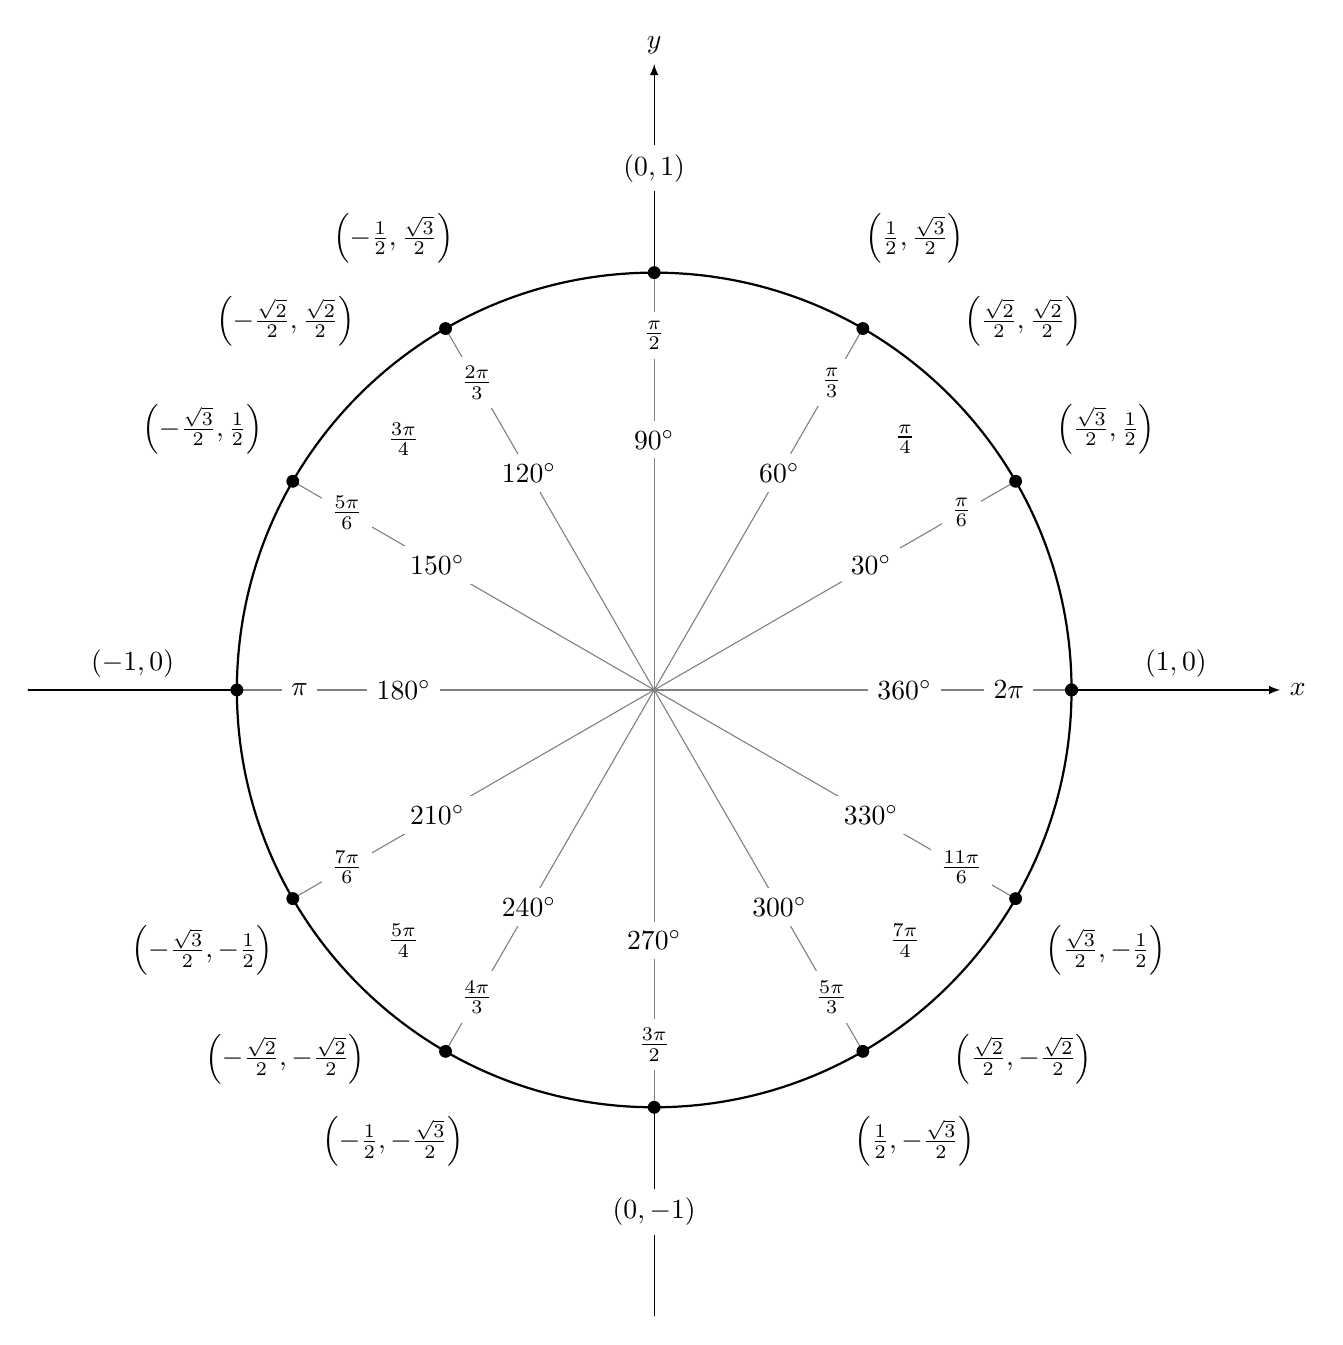
\begin{tikzpicture}[scale=5.3,cap=round,>=latex]
		% draw the coordinates
		\draw[->] (-1.5cm,0cm) -- (1.5cm,0cm) node[anchor=west,fill=white] {$x$};
		\draw[->] (0cm,-1.5cm) -- (0cm,1.5cm) node[anchor=south,fill=white] {$y$};

		% draw the unit circle
		\draw[thick] (0cm,0cm) circle(1cm);

		% lines from center to point
		\foreach \x in {0,30,...,360}
			\draw[gray] (0cm,0cm) -- (\x:1cm);

		% dots at each point
		\foreach \x in {0,30,...,360}
			\filldraw[black] (\x:1cm) circle(0.4pt);

		% draw each angle in degrees
		\foreach \x in {0,30,...,360}
			\draw (\x:0.6cm) node[fill=white] {$\x^\circ$};

		% draw each angle in radians
		\foreach \x/\xtext in {
		0,
		30/\frac{\pi}{6},
		45/\frac{\pi}{4},
		60/\frac{\pi}{3},
		90/\frac{\pi}{2},
		120/\frac{2\pi}{3},
		135/\frac{3\pi}{4},
		150/\frac{5\pi}{6},
		180/\pi,
		210/\frac{7\pi}{6},
		225/\frac{5\pi}{4},
		240/\frac{4\pi}{3},
		270/\frac{3\pi}{2},
		300/\frac{5\pi}{3},
		315/\frac{7\pi}{4},
		330/\frac{11\pi}{6},
		360/2\pi}
			\draw (\x:0.85cm) node[fill=white] {$\xtext$};

		% draw the coordinates for the first quadrant
		\foreach \x/\xtext/\y in {
		30/\frac{\sqrt{3}}{2}/\frac{1}{2},
		45/\frac{\sqrt{2}}{2}/\frac{\sqrt{2}}{2},
		60/\frac{1}{2}/\frac{\sqrt{3}}{2}}
			\draw (\x:1.25cm) node[fill=white] {$\left(\xtext,\y\right)$};

		% draw the coordinates for the second quadrant
		\foreach \x/\xtext/\y in {
		150/-\frac{\sqrt{3}}{2}/\frac{1}{2},
		135/-\frac{\sqrt{2}}{2}/\frac{\sqrt{2}}{2},
		120/-\frac{1}{2}/\frac{\sqrt{3}}{2}}
			\draw (\x:1.25cm) node[fill=white] {$\left(\xtext,\y\right)$};

		% draw the coordinates for the third quadrant
		\foreach \x/\xtext/\y in {
		210/-\frac{\sqrt{3}}{2}/-\frac{1}{2},
		225/-\frac{\sqrt{2}}{2}/-\frac{\sqrt{2}}{2},
		240/-\frac{1}{2}/-\frac{\sqrt{3}}{2}}
			\draw (\x:1.25cm) node[fill=white] {$\left(\xtext,\y\right)$};

		% draw the coordinates for the fourth quadrant
		\foreach \x/\xtext/\y in {
		330/\frac{\sqrt{3}}{2}/-\frac{1}{2},
		315/\frac{\sqrt{2}}{2}/-\frac{\sqrt{2}}{2},
		300/\frac{1}{2}/-\frac{\sqrt{3}}{2}}
			\draw (\x:1.25cm) node[fill=white] {$\left(\xtext,\y\right)$};

		% draw the horizontal and vertical coordinates
		% the placement is better this way
		\draw (-1.25cm,0cm) node[above=1pt,fill=white] {$\left(-1,0\right)$};
		\draw (1.25cm,0cm) node[above=1pt,fill=white] {$\left(1,0\right)$};
		\draw (0cm,-1.25cm) node[fill=white] {$\left(0,-1\right)$};
		\draw (0cm,1.25cm) node[fill=white] {$\left(0,1\right)$};
	\end{tikzpicture}
	\end{center}
\end{document}
